\section{Конструкторская часть}
В данном разделе представлены требования к программному обеспечению, рассмотрены алгоритмы, выбранные для построения сцены

\subsection{Требования к программному обеспечению}

Программа должна предоставлять графический интерфейс с функционалом:
\begin{itemize}
	\item задать спектральные характеристики добавляемого объекта;
	\item изменить положение объекта, положение камеры, положение источника света в пространстве;
	\item выбрать функции при процедурном текстурировании, рисунки из библиотеки при проективном текстурировании;
	\item моделировать неровную поверхность.
\end{itemize}

\subsection{Аппроксимация трёхмерных объектов}
В ходе работы программы активно используется полигональная сетка.
Это совокупность вершин, рёбер и граней, которые определяют форму многогранного объекта в трёхмерной компьютерной графике.
Недостатком этого метода является его приблизительность.
Правда, видимые недочёты можно исправить, сделав разбиение более детальным, но это приведёт к дополнительным затратам по памяти и временным затратам.

Примеры использования полигональной сетки приведены на рисунок \ref{fig:polygon}.

\begin{figure}[h]
	\centering
	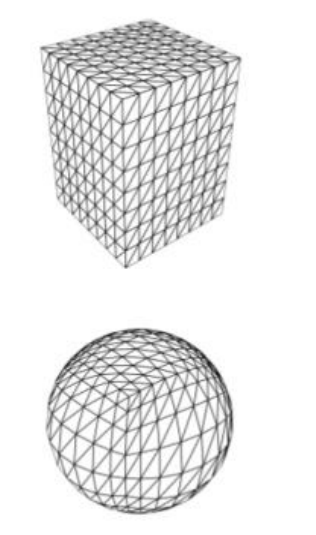
\includegraphics[width=0.3\textwidth]{img/polygon.png}
	\caption{Примеры использования полигональной сетки}
	\label{fig:polygon}
\end{figure}
\clearpage
В рамках текущей задачи в качестве граней выбраны треугольники.
Построение полигональной сетки осуществляется следующим образом:
\begin{enumerate}
	\item Kyб : зная число разбиений по осям, промежуточные точки вычисляются через ее предыдущую точку и шаги, которые задаются пользователем:
	\begin{equation}
		x = x + step_x, y = y + step_y, z = z_0
	\end{equation}
	\begin{equation}
		x = x_0, y = y + step_y, z = z + step_z
	\end{equation}
	\begin{equation}
		x = x + step_x, y = y_0, z = z + step_z
	\end{equation}
	где step\_x --- шаг разбиения по оси x, step\_y --- шаг разбиения по оси y, step\_z --- шаг разбиения по оси z.
	\item Цилиндр --- зная высота ${h}$ и радиус ${r}$, координаты вычисляются через цилиндрический параметр:
	\begin{equation}
		x = r * cos(\alpha), y = r * sin(\alpha), z = z_0
	\end{equation}
	где $0 \leqslant \alpha \leqslant 360$ ($\alpha$ в градусах), $-h \leqslant z_0 \leqslant h$.
	
	\item Сфера --- зная радиус ${r}$, координаты вычисляются через сферический параметр.
	\begin{equation}
		x = r * sin(\alpha) * cos(\beta), y = r * sin(\alpha) * sin(\beta), z = r * cos(\alpha)
	\end{equation}
	где $0 \leqslant \alpha \leqslant 180$, $0 \leqslant \beta \leqslant 360$ ($\alpha$, $\beta$ в градусах).
\end{enumerate}
Далее все полученные точки соединяются в треугольники.
\subsection{Общий алгоритм построения изображения}

Алгоритм генерации изображения представлен на рисунке~\ref{fig:alg_scene}.

\begin{figure}[h]
	\centering
	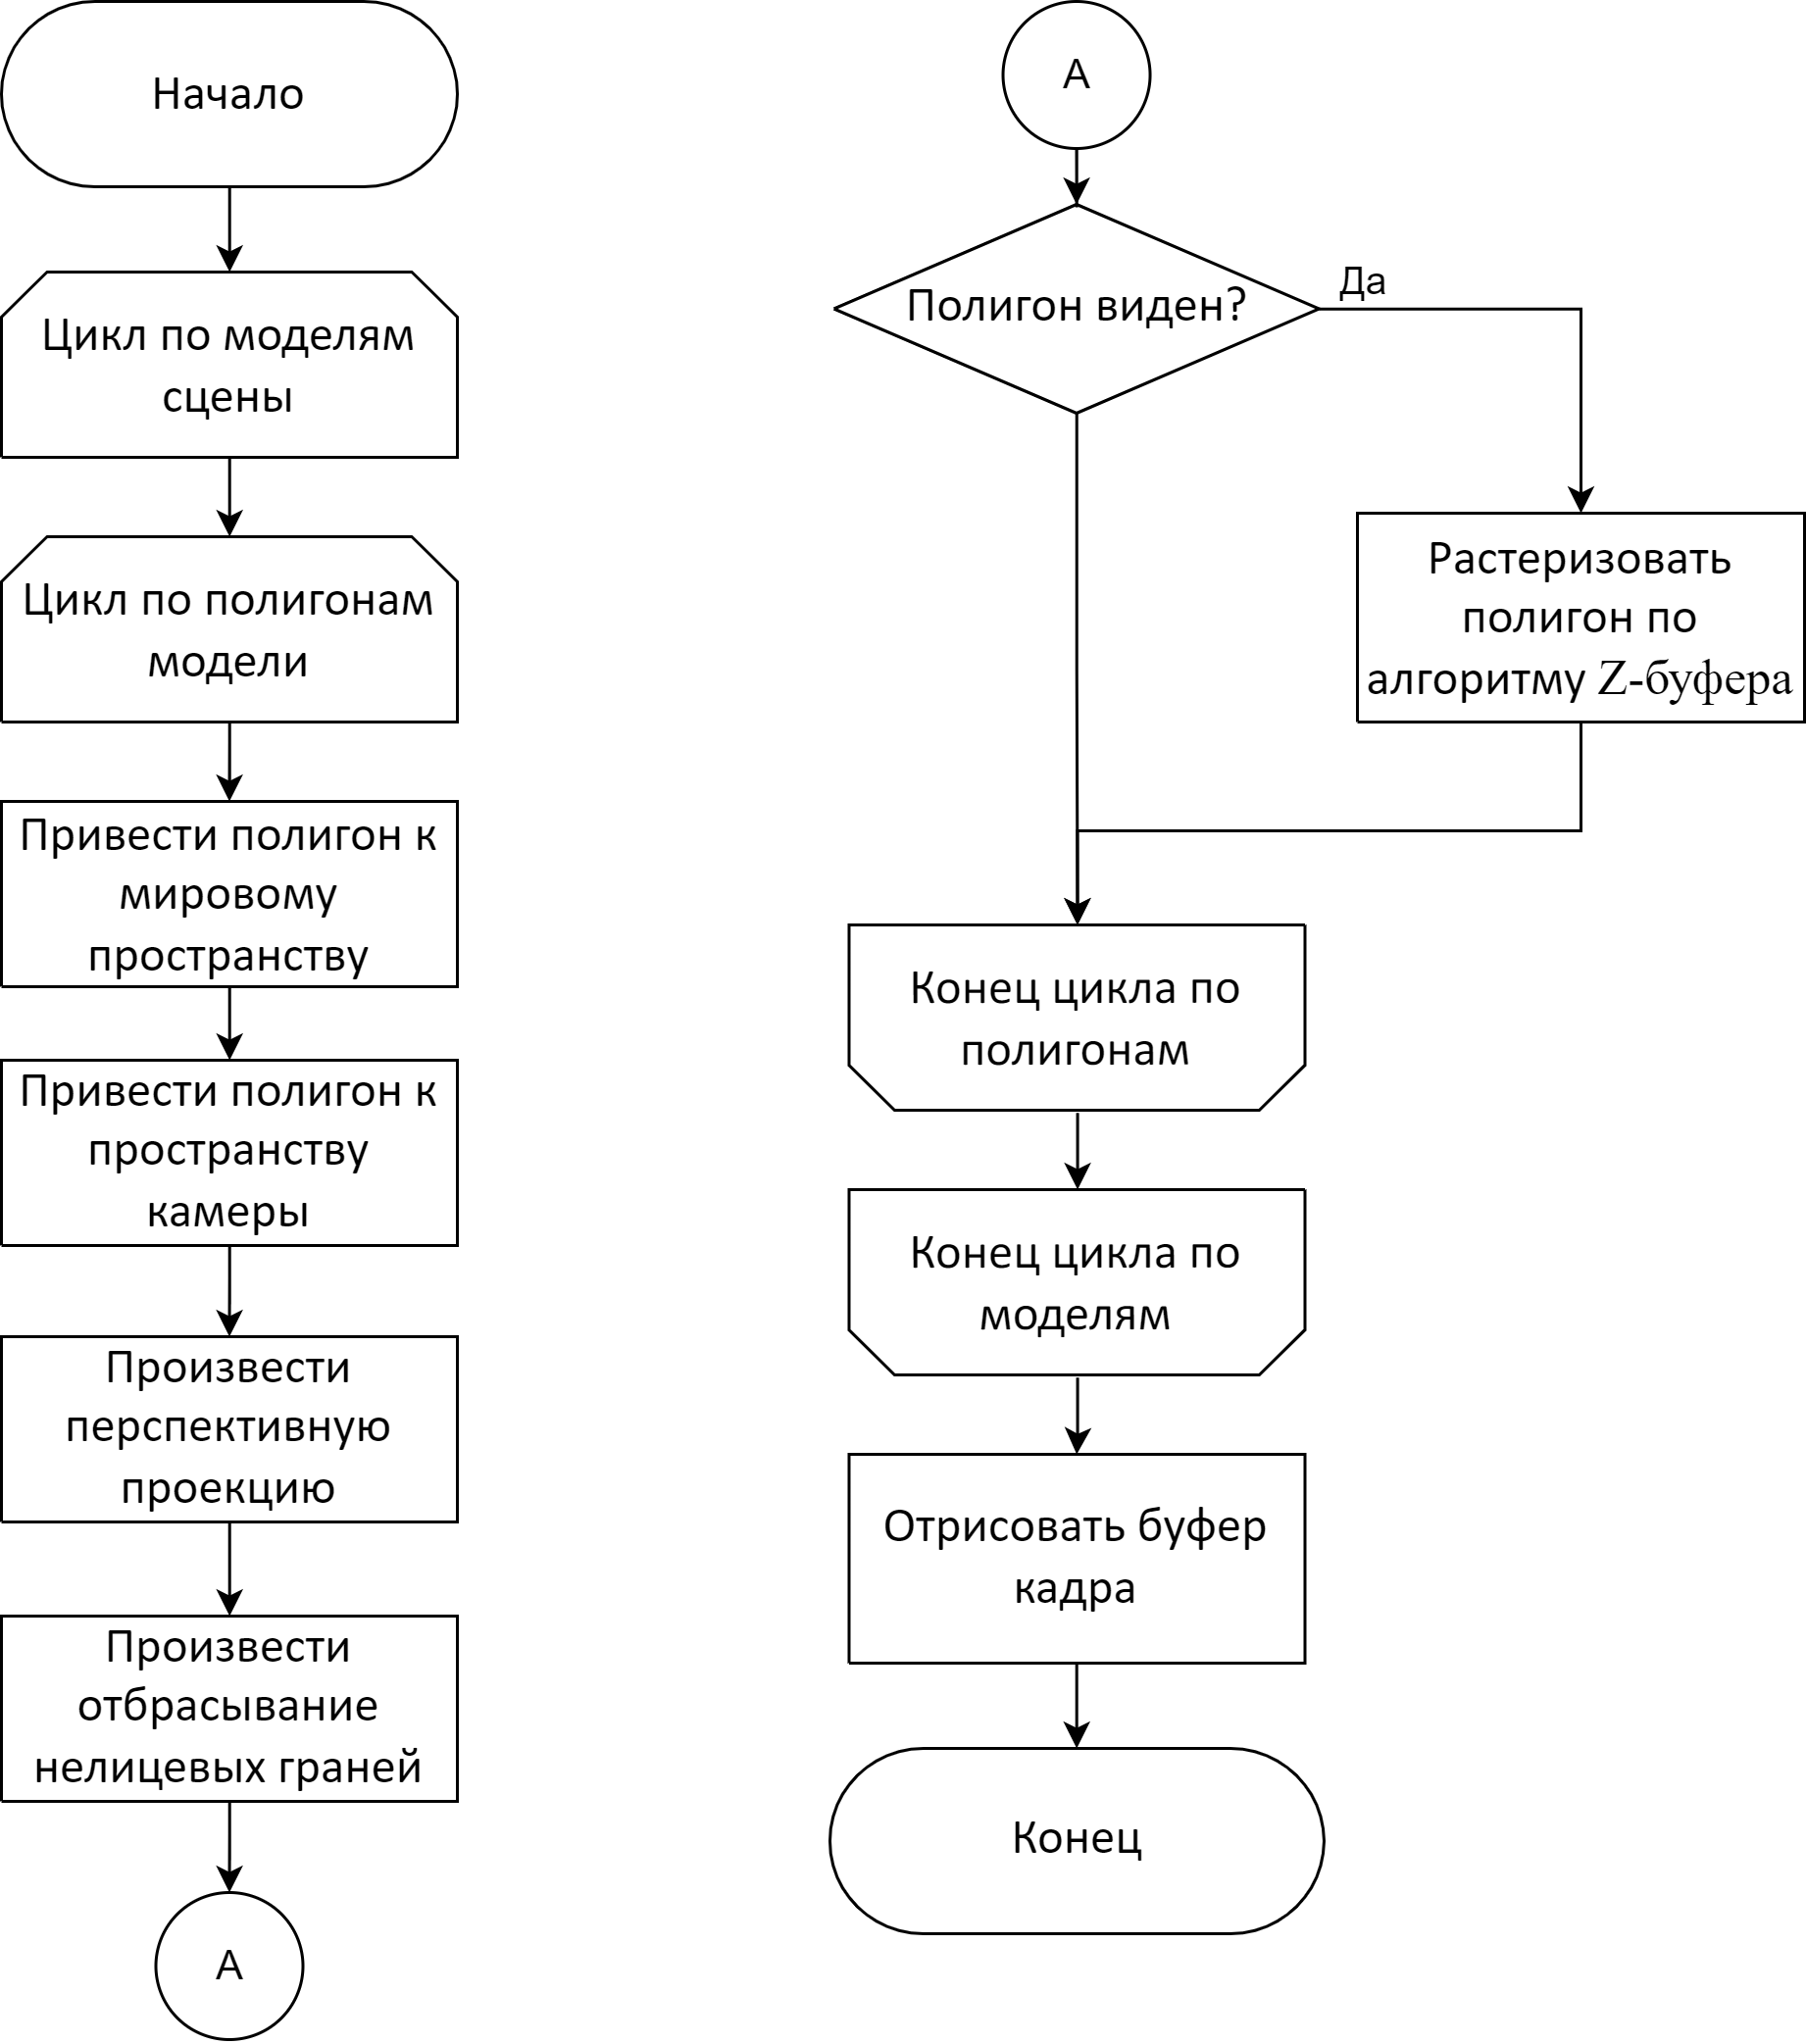
\includegraphics[width=0.8\textwidth]{img/algorithms/alg_scene.png}
	\caption{Общая схема алгоритма синтеза изображения}
	\label{fig:alg_scene}
\end{figure}

\clearpage

\subsection{Алгоритм Z-буфера}

Для растеризации треугольного полигона сначала необходимо найти ограничивающий его прямоугольник, в котором этот полигон содержится. 
Это делается для того, чтобы не тратить время на растеризацию пикселей, не являющихся частью полигона.
Затем для каждого пиксела ограничивающего прямоугольника находятся его барицентрические координаты относительно вершин полигона.

Затем производится сравнение значения глубины точки со значением глубины из Z-буфера. Если глубина пикселя меньше, значит он лежит ближе к камере и должен быть растеризован. Происходит вычисление интенсивности пикселя, его значение заносится в буфер кадра, а в Z-буфер заносится значение глубины пиксела.

Полная схема алгоритма Z-буфера представлена на  рисунке~\ref{fig:z-buffer}.

\begin{figure}[h]
	\centering
	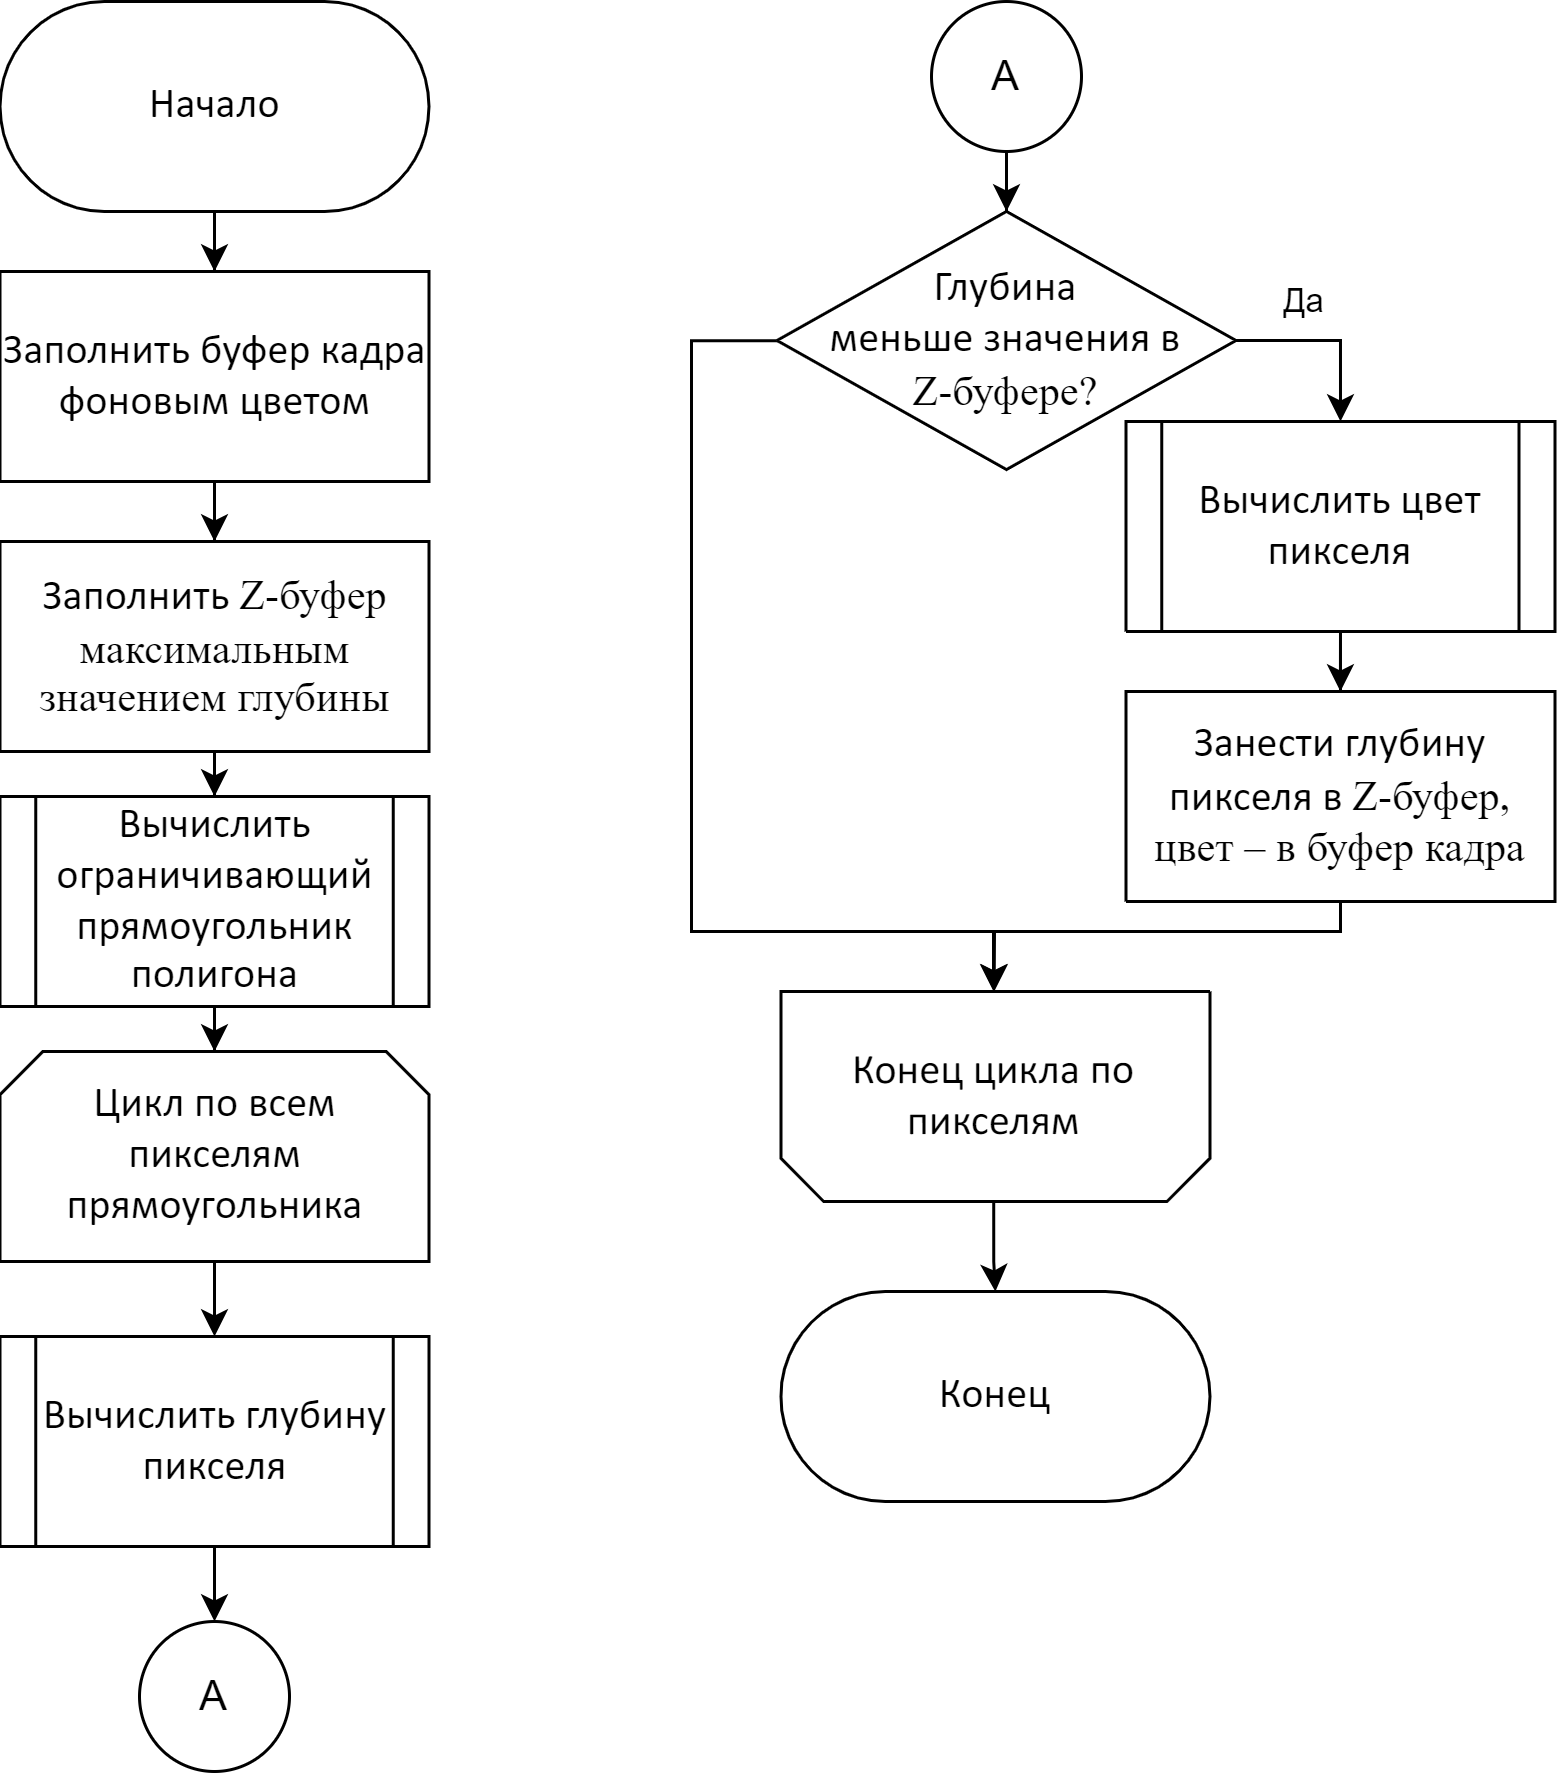
\includegraphics[width=0.8\textwidth]{img/algorithms/alg-z-buffer.png}
	\caption{Схема алгоритма Z-буфера}
	\label{fig:z-buffer}
\end{figure}
\clearpage

\subsection{Описание трёхмерных преобразований}
\subsubsection{Способ хранения декартовых координат}
Координаты можно хранить в форме вектор-столбца [x, y, z].
Однако в этом случае неудобно применять преобразования, так такой вектор нельзя умножить на соответствующие матрицы трансформации размерности четыре.
Целесообразнее использовать вектор-столбцы размерности четыре [x, y, z, w], где w для точки равно одному.
Преобразования координат выполняются умножением слева преобразуемого вектора-столбца на соответствующую матрицу линейного оператора.

\subsubsection{Аффинные преобразования}

В представленном алгоритме синтеза изображения первым этапом преобразования полигона пред его растеризацией является переход модели в мировое пространство. 
Такое действие осуществляется с помощью матриц аффинных преобразований.
В данном курсовом проекте над объектами возможно произвести следующие операции.

\begin{itemize}
	\item Поворот вокруг координатных осей описывается углом $\alpha$ и осью вращения.
	Матрица поворота имеет вид:
	\begin{itemize}
		\item вокруг оси OX:
		\begin{equation}
			\begin{pmatrix}
				1 	& 0 		  & 0 	       & 0 \\
				0 	& cos \alpha  & sin \alpha & 0 \\
				0	& -sin \alpha & cos \alpha & 0 \\
				0 	& 0 		  & 0          & 1
			\end{pmatrix}
		\end{equation}
		\item вокруг оси OY:
			\begin{equation}
			\begin{pmatrix}
				cos \alpha 	& 0 & -sin \alpha & 0 \\
				0 			& 1 & 0 		  & 0 \\
				sin \alpha	& 0 & cos \alpha  & 0 \\
				0 			& 0 & 0           & 1
			\end{pmatrix}
		\end{equation}
		\item вокруг оси OZ:
		\begin{equation}
			\begin{pmatrix}
				cos \alpha 	 & sin \alpha & 0 & 0 \\
				-sin \alpha  & cos \alpha & 0 & 0 \\
				0	 		 & 0		  & 1 & 0 \\
				0 			 & 0 		  & 0 & 1
			\end{pmatrix}
		\end{equation}
	\end{itemize}
	\item Перенос в трехмерном пространстве задается значения вдоль координатных осей OX, OY, OZ --- dx, dy, dz соответственно.
	Матрица переноса имеет вид:
	\begin{equation}
		\begin{pmatrix}
			1  & 0  & 0  & 0 \\
			0  & 1  & 0  & 0 \\
			0  & 0  & 1  & 0 \\
			dx & dy	& dz & 1
		\end{pmatrix}
	\end{equation}
\end{itemize}

\subsubsection{Преобразования трёхмерной сцены в пространство камеры}
Чтобы привести трёхмерную сцену к пространству камеру, нужно умножить каждую вершину всех полигональных моделей на матрицу камеры. 
Сама же камера задаётся аргументами: положение камеры в мировом пространстве, вектор наблюдения взгляда, направление верха камеры.
Пусть:
$\alpha$ – координаты точки в пространстве, на которую смотрит камера, 
$\beta$ – вектор, который указывает, куда смотрит верх камеры,
$\psi$– ортогональный вектор к векторам направления взгляда и вектору направления.

Тогда матрица будет выглядеть так:
\begin{equation*}
	A = \left(
	\begin{array}{cccc}
		\alpha_x & \beta_x & \psi_x & 0\\
		\alpha_y & \beta_y & \psi_y & 0 \\
		\alpha_z & \beta_z & \psi_z & 0 \\
		-(P*\alpha) & -(P*\beta) &-(P*\psi) & 1
	\end{array}
	\right)
\end{equation*}

\subsubsection{Матрица перспективной проекции}
После перехода в пространство камеры нужно умножить каждую вершину всех полигонов на матрицу проекции. 
Эта матрица преобразует заданный диапазон усечённой пирамиды в пространство отсечения, и изменяет w-компоненту так, что чем дальше от наблюдателя находится вершина, тем больше возрастает $ w $. 
После преобразования координат в пространство отсечения, координаты x и y попадают в промежуток [$-w$, $w$], а вершина $z$ – [-0, $w$]. 
Всё, что находится вне диапазона, отсекается.

Пусть AR – отношение ширины изображения к его высоте, $\alpha$ – угол обзора камеры, $Z_n$ – координата $z$ ближайшей к камере плоскости отсечения пирамиды видимости, 
$ Z_f $ – координата $z$ дальней от камеры плоскости отсечения пирамиды видимости. 
Тогда матрица перспективной проекции принимает вид:
\begin{equation*}
	A = \left(
	\begin{array}{cccc}
		\frac{cot(\frac{\alpha}{2})}{AR} & 0 & 0 & 0\\
		0 & cot(\frac{\alpha}{2}) & 0 & 0 \\
		0 & 0 & \frac{Z_f \times Z_n}{Z_f - Z_n} & 1 \\
		0) & 0 & \frac{Z_f}{Z_f - Z_n} & 0
	\end{array}
	\right)
\end{equation*}
Следующий этап – спроецировать все координаты на одну плоскость, разделив всё на координату $z$. После умножения вектора координат на матрицу перспективной проекции, реальная координата $z$ заносится в w-компоненту, так что вместо деления на $z$ делят на $w$.

\subsection{Процедурные текстуры}
Процедурные текстуры --- это тектсуры, описываемые математическими формулами. Такие текстуры не занимают в памяти места, а создаются, например, пиксельным шейдером.

Преимуществом процедурных текстур является неограниченный уровень детализации каждой тектсуры (пикселизации не будет, так как текстура всегда генерируется под необходимый для её отображения размер). Недостатком процедурных текстура можно назвать тот случай, когда подобранная функция является сложной, так как зависит от большого числа переменных.

Необходимо найти функцию C(X,Y,Z), определяющую для каждой точки поверхности цвет таким образом, чтобы он соответствовал цвету моделируемого материала (наносимого рисунка). Такой подход не требует больших затрат памяти и хорошо работает с поверхностями любой сложности. Но поскольку используемая функция зависит от большого количества параметров, то возникают сложности в подборе этой функции, с другой стороны, изменение этих параметров позволяет легко изменять свойства текстуры.

\subsection{Проективные текстуры}
Суть моделирования проективных тектсур заключается в том, что текстуры проецируются на поверхность параллельным переносом (плосоке проецирование), либо цилиндрическим и сферическим методами.
Недостатки проективных текстур - большой объем памяти для хранения образцов текстур, небольшая гибкость и трудность текстурирования объектов сложной формы. 

Задается в некоторой (обычно двумерной) системе координат рисунок, подлежащий нанесению на трехмерную поверхность.
Тогда для наложения заданного рисунка на поверхность необходимо найти функцию отображения или, другими словами, произвести преобразование координат.
Проективным текстурам присущи определенные недостатки:
\begin{itemize}
	\item для хранения используемых изображений требуется достаточно большой объем памяти;
	\item они не обладают гибкостью;
	\item возможны большие сложности при подборе способа проектирования при нанесении рисунка на объекты сложной формы.
\end{itemize}

\subsection{Моделирование неровностей}
%Пусть Q(X,Y) – уравнение поверхности, т.е. функция Q позволяет для каждой точки поверхности определить ее третью координату Z. В произвольной точке поверхности частные производные по направлениям X,Y лежат в плоскости, касательной к поверхности в этой точке. Нормаль в точке поверхности может определяться векторным произведением этих производных:
%\begin{equation}
%	N = [Q'_x, Q'_y]
%\end{equation}

Для создания шероховатой поверхности можно создать новую поверхность путем внесения возмущения в направлении нормали в точках поверхности \cite{roders}.

В данной работе тела аппроксимируются треугольниками, затем треугольники растеризуются с помощью барицентрического координата.
Поэтому возмущение вносится в нормаль каждой вершины треугольника.

Нормали поверхности, состоящей из трех точек A, B, C определяется векторным произведением:
\begin{equation}
	\overrightarrow n_{ABC} = [\overrightarrow {AB}, \overrightarrow {AC}]
\end{equation}
\begin{equation}
	 \overrightarrow n_A = \overrightarrow n_B = \overrightarrow n_C = \overrightarrow n_{ABC}
\end{equation}

Вектор возмущение вычисляется случайным образом, затем сложится с вектором нормали в каждой вершине.
Новая нормаль вычисляется следующим образом:
\begin{equation}
	\overrightarrow n' = (sin(random()), cos(random()), sin(2 * random()))
\end{equation}
\begin{equation}
	\overrightarrow n_A= \overrightarrow n_A + \overrightarrow n'
\end{equation}

Результирующий вектор после сложения нормализуется и этот вектор записывается в каждую вершину в качестве новой нормали.
\begin{equation}
	\overrightarrow n_A = \frac{\overrightarrow n_A}{|\overrightarrow n_A|}
\end{equation}
$ $

Полная схема алгоритма моделирования неровностей представлена на  рисунке~\ref{fig:bump}.
\clearpage
\begin{figure}[h]
	\centering
	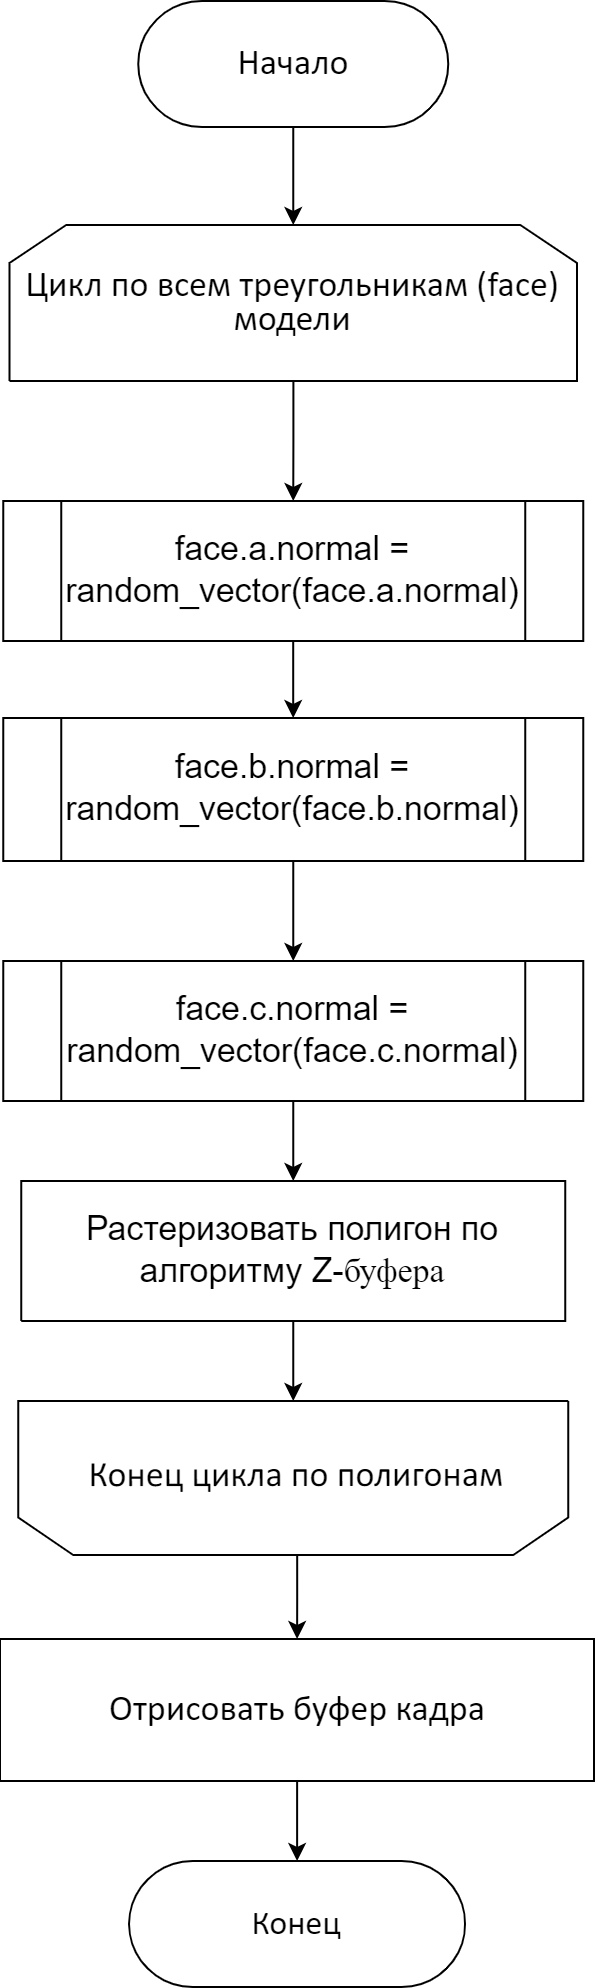
\includegraphics[width=0.4\textwidth]{img/algorithms/bump.png}
	\caption{Схема алгоритма моделирования неровностей}
	\label{fig:bump}
\end{figure}
\clearpage
\subsection*{Вывод}
Были описаны требования к программному обеспечению, алгоритмы для построения сцены в пространстве изображения, изменения положения объекта в пространстве, построение камеры и ее проекций. Также описаны процедурные текстуры, проективные текстуры и алгоритм моделирования неровностей.